%%%%%%%%%%%%%%%%%%%%%%%%%%%%%%%%%%%%%%%%%%%%%%%%%%%%%%%%%%%%%%%%%%%%%%%%%%%%%%%%
%2345678901234567890123456789012345678901234567890123456789012345678901234567890
%        1         2         3         4         5         6         7         8

\documentclass[letterpaper, 10 pt, conference]{ieeeconf}  % Comment this line out
                                                          % if you need a4paper
%\documentclass[a4paper, 10pt, conference]{ieeeconf}      % Use this line for a4
                                                          % paper

\IEEEoverridecommandlockouts                              % This command is only
                                                          % needed if you want to
                                                          % use the \thanks command
\overrideIEEEmargins
% See the \addtolength command later in the file to balance the column lengths
% on the last page of the document

\usepackage[utf8]{inputenc}
\usepackage[T1]{fontenc}

% The following packages can be found on http:\\www.ctan.org
\usepackage{graphicx} % for pdf, bitmapped graphics files
%\usepackage{epsfig} % for postscript graphics files
%\usepackage{mathptmx} % assumes new font selection scheme installed
%\usepackage{mathptmx} % assumes new font selection scheme installed
\usepackage{amsmath} % assumes amsmath package installed
%\usepackage{amssymb}  % assumes amsmath package installed

\title{\LARGE \bf
Lab3: Assembly the robot and testing actuators
}

%\author{ \parbox{3 in}{\centering Huibert Kwakernaak*
%         \thanks{*Use the $\backslash$thanks command to put information here}\\
%         Faculty of Electrical Engineering, Mathematics and Computer Science\\
%         University of Twente\\
%         7500 AE Enschede, The Netherlands\\
%         {\tt\small h.kwakernaak@autsubmit.com}}
%         \hspace*{ 0.5 in}
%         \parbox{3 in}{ \centering Pradeep Misra**
%         \thanks{**The footnote marks may be inserted manually}\\
%        Department of Electrical Engineering \\
%         Wright State University\\
%         Dayton, OH 45435, USA\\
%         {\tt\small pmisra@cs.wright.edu}}
%}

\author{Yiwen(Robert) Wu\\\\https://github.com/Robert1124/cse460}


\begin{document}



\maketitle
\thispagestyle{empty}
\pagestyle{empty}

\section{Part1: Assemble the robot}
We assembled the robot following the instruction.

\begin{figure}[htbp]
    \centering
    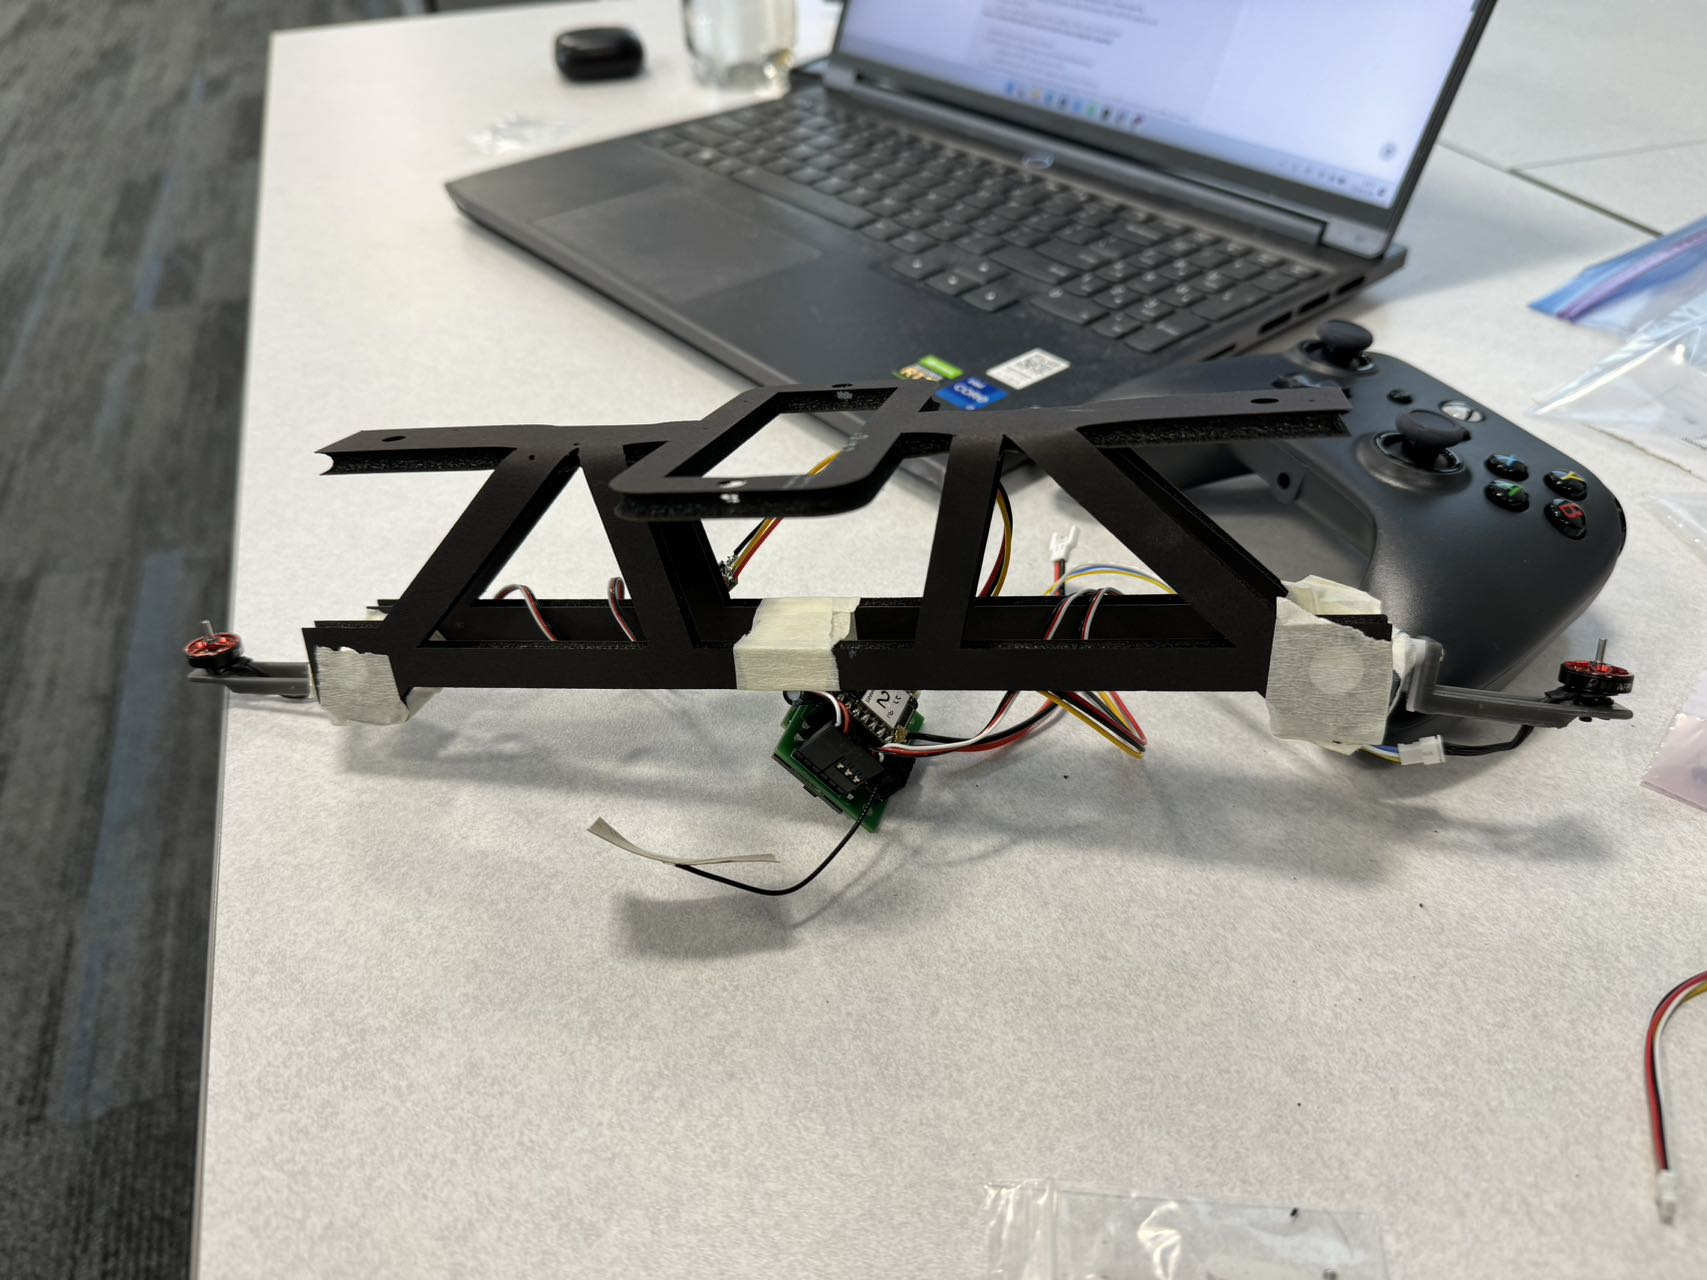
\includegraphics[width=0.4\textwidth]{image1.jpg}
\end{figure}

Here are 5 ways to improve the design:

1. Use plastic to make the frame. The materials used now are too fragile. Several times while I was adjusting the shape of this frame I was afraid I was going to break the frame to pieces.

2. There should be a better way to fix the motors. The sides of the motors can be held well, but the back of the motor does not have a proper support point for us to fix it.

3. To faster assemble the robot, I suggest to fix the motor to one side first, then bend and tied the frame and fix the motor to the other side.

4. There should be a position to place ESP32 well on the frame.

5. There should be a structure horizontal to the main frame to help keep the balance.
\newpage
\section{Part3: Control the actuators}

After we run the RawBicopter.py and moved the left vertical joystick, the LED turned on. It was not successful every time, we needed to reconnect it again and again to reduce the delay.

Then, we wanted to test two servos and two motors. At first, we set the firmware correctly and the python code was also correct, however, nothing happened after we moved the joystick. We found the wire was wrong connected, so we reconnected wires in correct way and successfully test the servos and motors. We matched the two servos with the two axis and the button A with the both motors.

With the axis and button A, we flied the robot with helium balloon and controlled it with the joystick.

\begin{figure}[htbp]
    \centering
    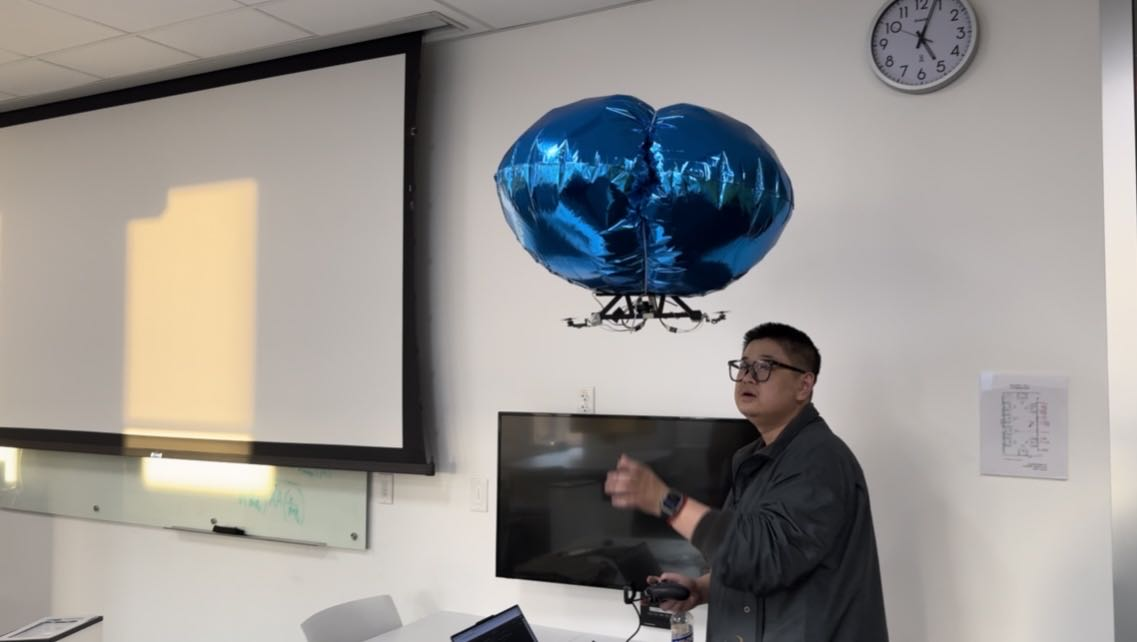
\includegraphics[width=0.4\textwidth]{image2.jpg}
\end{figure}

\end{document}
